\section{Archetypes}
\note{
    \begin{itemize}
        \item \textbf{During our work, we found many different approaches to randomness beacons.}
				\item We have \textbf{generalized} these approaches and \textbf{boiled them down to 3 archetypes}, which are \textbf{broad characterizations} of \textbf{prominent} ways of creating a randomness beacons.
				\item These archetypes enables us to \textbf{generalize} over the approaches, \textbf{instead of treating each approach individually}.
    \end{itemize}
}

\begin{frame}{3 Archetypes}
    \newlength{\onethird}
    \setlength{\onethird}{0.315\textwidth}
    \vspace{.2cm}
    \begin{minipage}[t]{\onethird}
        \centering
        \textbf{Autocratic Collector\vphantom{j}}\\
        \vspace{.6cm}
        \scalebox{0.8}{
        \begin{tikzpicture}[auto]
            \pgfdeclarelayer{background}
            \pgfsetlayers{background,main}
            \node[block] (input) {Private external\\entropy source};
            \node[block, below=1cm of input] (computation) {Computation\\$f(I_t)$};
            \node[block, below=1cm of computation] (users) {Users};
            \draw[arrow] (input) -- node (inp) {$I_t$} (computation);
            \draw[arrow] (computation) -- node {$O_t$} (users);
            \begin{pgfonlayer}{background}
                %\node[block] (beacon) [container, fit={(input) (computation)}] {};
            \end{pgfonlayer}
        \end{tikzpicture}
        }
    \end{minipage}
    ~~\begin{minipage}[t]{\onethird}
        \centering
        \textbf{Specialized MPC}\\
        \vspace{.6cm}
        \scalebox{0.8}{
        \begin{tikzpicture}[auto]
            \pgfdeclarelayer{background}
            \pgfsetlayers{background,main}
            \node[block] (input) {Each user's input};
            \node[block, text width=9em, below=1cm of input] (computation) {Partial computation\\$f'(I'_t)$};
            \node[block, below=1cm of computation] (users) {Users};
            \draw[arrow] (input) -- node (inp) {$I_{u,t}$} (computation);
            \draw[arrow] (computation) -- node {$O_t$} (users);
            \draw[arrow] (computation.south) to [out=250, in=250, looseness=2] node[shift={(-7mm,3mm)}] (rprime) {$O'_t$} ([shift={(-10mm,0mm)}]computation.south);
            \begin{pgfonlayer}{background}
                %\node[block] (beacon) [container, fill=GoogleLightBlue!40, draw=GoogleLightBlue, fit={(input) (computation) ([shift={(0mm,3mm)}]rprime.south west)}] {};
            \end{pgfonlayer}
        \end{tikzpicture}
        }
    \end{minipage}
    ~~\begin{minipage}[t]{\onethird}
        \centering
        \textbf{Transparent Authority}\\
        \vspace{.6cm}
        \scalebox{0.8}{
        \begin{tikzpicture}[auto]
            \pgfdeclarelayer{background}
            \pgfsetlayers{background,main}
            \node[block] (input) {Verifiable input};
            \node[block, below=1cm of input] (computation) {Computation\\$f(I_t)$};
            \node[block, below=1cm of computation] (users) {Users};
            \draw[arrow] (input) -- node (inp) {$I_t$} (computation);
            \draw[arrow] (computation) -- node {$O_t$} (users);
            \begin{pgfonlayer}{background}
                %\node[block] (beacon) [container, fill=GoogleBlueGrey!40, draw=GoogleBlueGrey, fit={(computation)}] {};
            \end{pgfonlayer}
        \end{tikzpicture}
        }
    \end{minipage}
\end{frame}
\note{
	\begin{multicols}{2}
    \begin{itemize}
        %So these are our three archetypes.
				\item Autocratic Collector
				\begin{itemize}
					\item Characterized by users need to trust.
				\end{itemize}
				\item Specialized MPC
				\begin{itemize}
					\item \textbf{alleviates need for trust} in an autocratic collector
					\item Characterized by: Partial Computation by \textbf{all} participants
					\item each user input: private number (so random, that others can't predict it)
					\item However, sequentially is \textbf{not scalable}.
					\begin{itemize}
						\item We have \textbf{not seen} the classic sequential mpc.
						\item The\textbf{ two types} we have seen \textrightarrow{} \textbf{more advanced}
						\item But the figure captures the gist
					\end{itemize}

				\end{itemize}
				\item Transparent Authority
				\begin{itemize}
					\item \textbf{Characterized by full transparency} in sourcing \textbf{input} and execution of \textbf{computation}
					\item \textbf{Output} can be \textbf{verified} to make sure it is really random
					%\item In case of user input, users want to check that their input was part of computation
					\item This is the \textbf{largest archetype} in terms of literature.
					\item 3.00
				\end{itemize}
		\end{itemize}
	\end{multicols}
}

\begin{frame}{Autocratic Collector: The NIST Beacon}
    \begin{columns}
        \begin{column}{0.7\textwidth}
						\vspace{.5cm}
            \begin{itemize}
                \item \textsc{\textbf{Input:}} Output from a photon splitter
								\item \textsc{\textbf{Computation:}} Crypto-hardened?
                \item \textsc{\textbf{Output:}} 512 bits every 60 seconds
								%\begin{itemize}
								%  \item The output at January 17, 15:11 (UTC)\\
								%	      \texttt{\scriptsize 67AE66B6E1812F4D32064B834A5E1AD5\\1424DCBC18DF8A9AAE2B8B7FA409002E\\9E314045F6E595A8EEBBB027CFBB4D8B\\BA64007F6EAE3EC92051ADD8391DA2B9\\}
								%\end{itemize}

            \end{itemize}
						\vspace{.7cm}\centering
						{%
							\setlength{\fboxsep}{0pt}%
							\setlength{\fboxrule}{.75pt}%
							\fbox{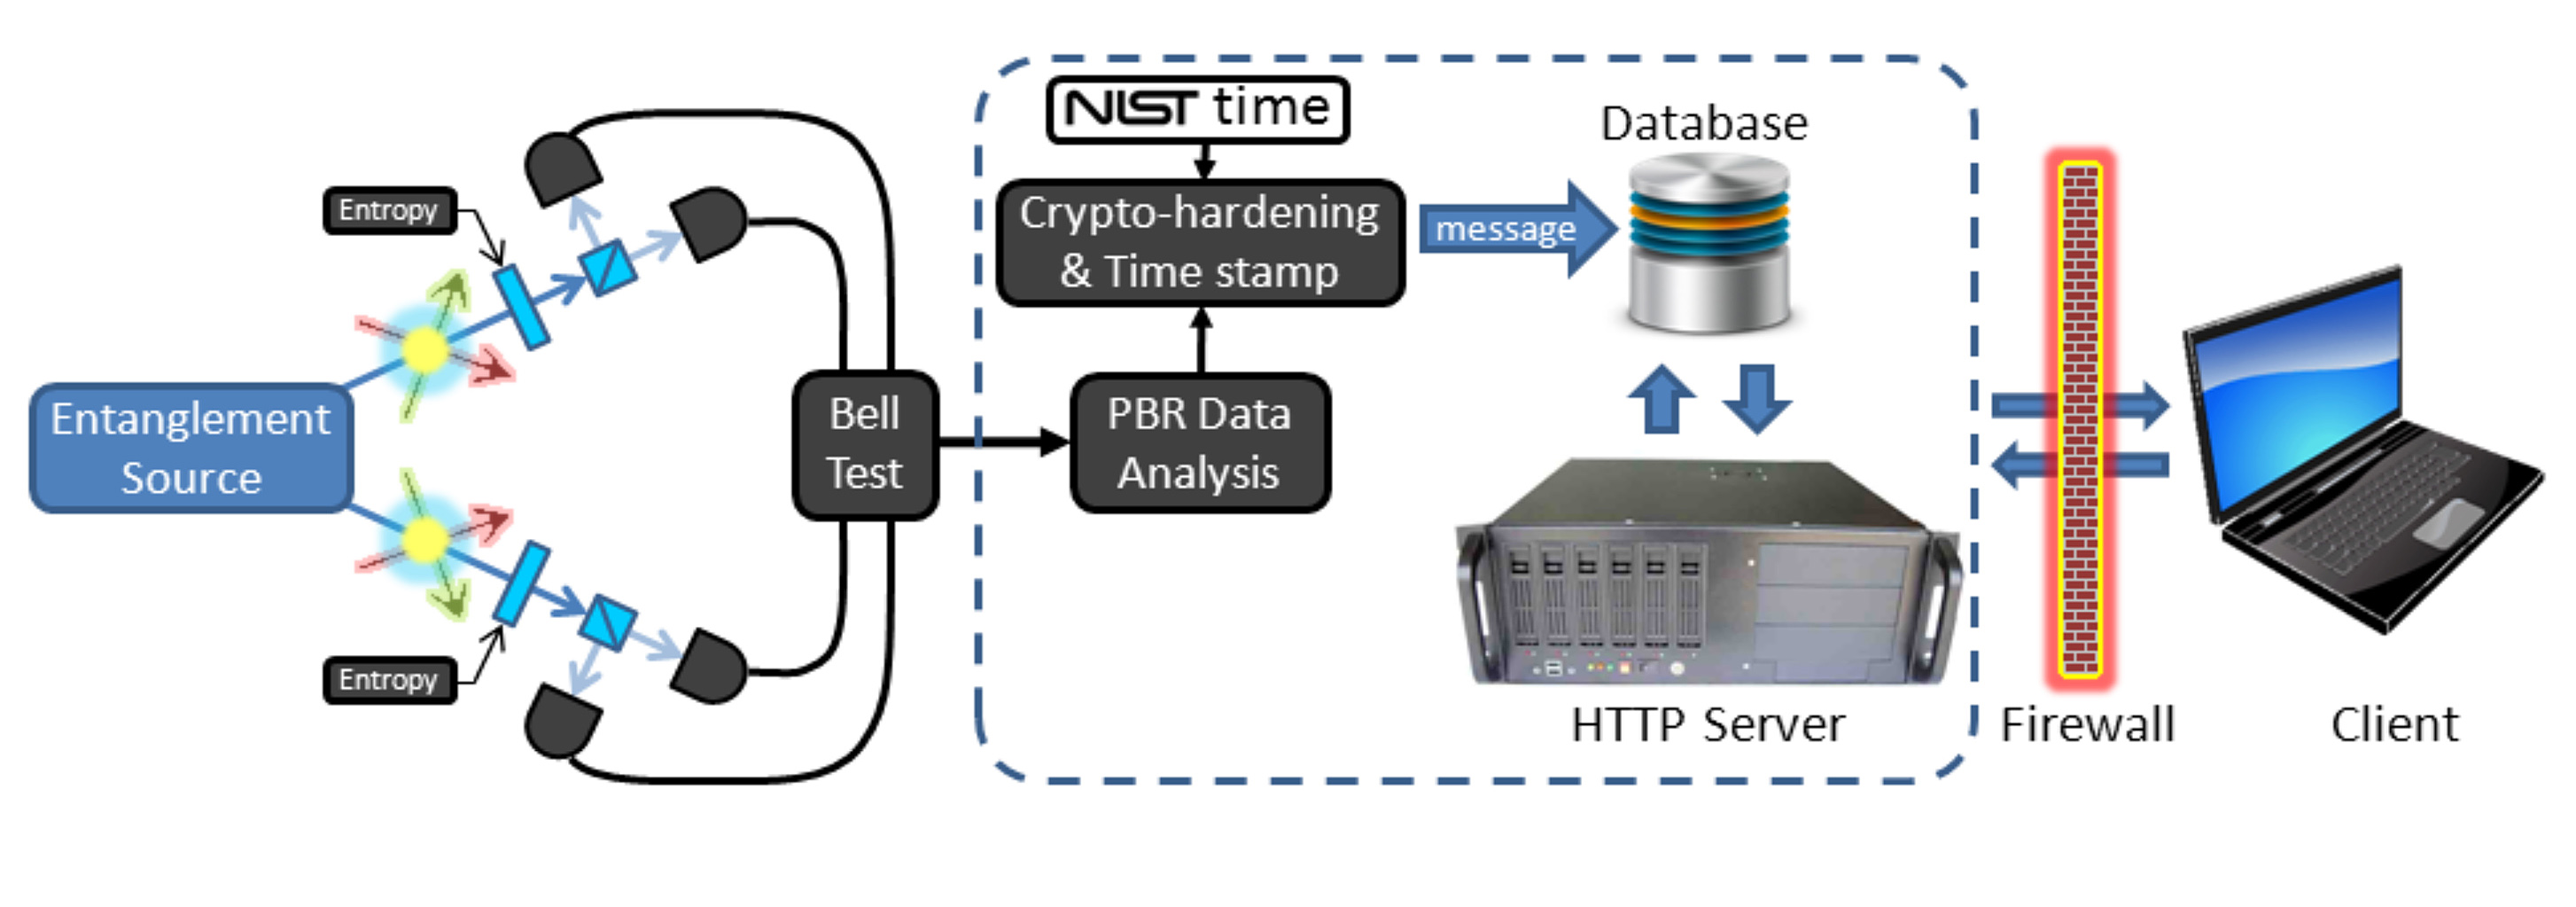
\includegraphics[width=.95\textwidth]{figures/nist.jpg}}\\
							\tiny
							\vspace{-1.5em}Image source: NIST%
						}%
        \end{column}
        \begin{column}{0.3\textwidth}
            \begin{center}
                \scalebox{0.85}{
                \begin{tikzpicture}[auto]
                    \pgfdeclarelayer{background}
                    \pgfsetlayers{background,main}
                    \node[block] (input) {Private external\\entropy source};
                    \node[block, below=.7cm of input] (computation) {Computation\\$f(I_t)$};
                    \node[block, below=1.2cm of computation] (users) {Users};
                    \draw[arrow] (input) -- node (inp) {$I_t$} (computation);
                    \draw[arrow] (computation) -- node[yshift=-1mm] {$O_t$} (users);
                    \begin{pgfonlayer}{background}
                        \node[block] (beacon) [container, fit={(input) (computation)}] {};
                    \end{pgfonlayer}
                \end{tikzpicture}
                }
             \end{center}
        \end{column}
    \end{columns}

\end{frame}
\note{
    \begin{itemize}
        \item The only approach that is implemented and usable in a wide setting.
				\item NIST is run by the US government
				\begin{itemize}
					\item \textbf{claims} to generate the random number by observing \textbf{quantum-mechanical effects in a photon splitter}.
					\item \textbf{Every minute:} Outputs 512 unpredictable bits.
					\item Each output is "crypto hardened", whatever that means.
				\end{itemize}
				\item 4.15
    \end{itemize}
}

\begin{frame}{Specialized MPC: RandHerd}
    \begin{columns}
        \begin{column}{0.7\textwidth}
						Setup (10 minutes) + Round execution (6 seconds) \vspace{1cm}
						\\
						\textsc{\textbf{Hierarchy:}}
						\footnotesize
						\Tree [.{Protocol Leader} [.{Group Leader 1} $p_1$ $p_2$ $p_3$ ]
																			[.{Group Leader 2} $p_1$ $p_2$ $p_3$ ]
																			[.{Group Leader 3} $p_1$ $p_2$ $p_3$ ]
									]

        \end{column}
        \begin{column}{0.3\textwidth}
            \begin{center}
                \scalebox{0.85}{
                \begin{tikzpicture}[auto]
                    \pgfdeclarelayer{background}
                    \pgfsetlayers{background,main}
                    \node[block] (input) {Each user's input};
                    \node[block, text width=9em, below=.7cm of input] (computation) {Partial computation\\$f'(I'_t)$};
                    \node[block, below=1.7cm of computation] (users) {Users};
                    \draw[arrow] (input) -- node (inp) {$I_{u,t}$} (computation);
                    \draw[arrow] (computation) -- node[yshift=-5mm] {$O_t$} (users);
                    \draw[arrow] (computation.south) to [out=250, in=250, looseness=2] node[shift={(-7mm,3mm)}] (rprime) {$O'_t$} ([shift={(-10mm,0mm)}]computation.south);
                    \begin{pgfonlayer}{background}
                        \node[block] (beacon) [container, fill=GoogleLightBlue!40, draw=GoogleLightBlue, fit={(input) (computation) ([shift={(0mm,3mm)}]rprime.south west)}] {};
                    \end{pgfonlayer}
                \end{tikzpicture}
                }
             \end{center}
        \end{column}
        \end{columns}
\end{frame}
\note{
    \begin{itemize}
				\item RandHerd, Which consists of two parts.
				\begin{itemize}
					\item \textbf{Setup-part} where partcipants are \textbf{sharded} into a protocol leader, group leaders and participants. This takes roughly 10 minutes (n=1024).
					\item After the setup, participants can in the \textbf{round execution} can \textbf{generate} a random number \textbf{every 6 seconds.}
					\item \textbf{Participants}: random numbers \textrightarrow{} \textbf{batched} by group leaders \textrightarrow{} \textbf{collected} by protocol leader.
					\item \textbf{After some cryptographic computation} in batches back and forth between the protocol leader, group leaders, and ordinary participants, a \textbf{single collectively} created random number is \textbf{released} by the protocol leader.
					\item This number is efficiently \textbf{verifiable} by everyone.
					\item 5.45
				\end{itemize}
    \end{itemize}
}

\begin{frame}{Transparent Authority: A Random Zoo}
    \begin{columns}
        \begin{column}{0.7\textwidth}
            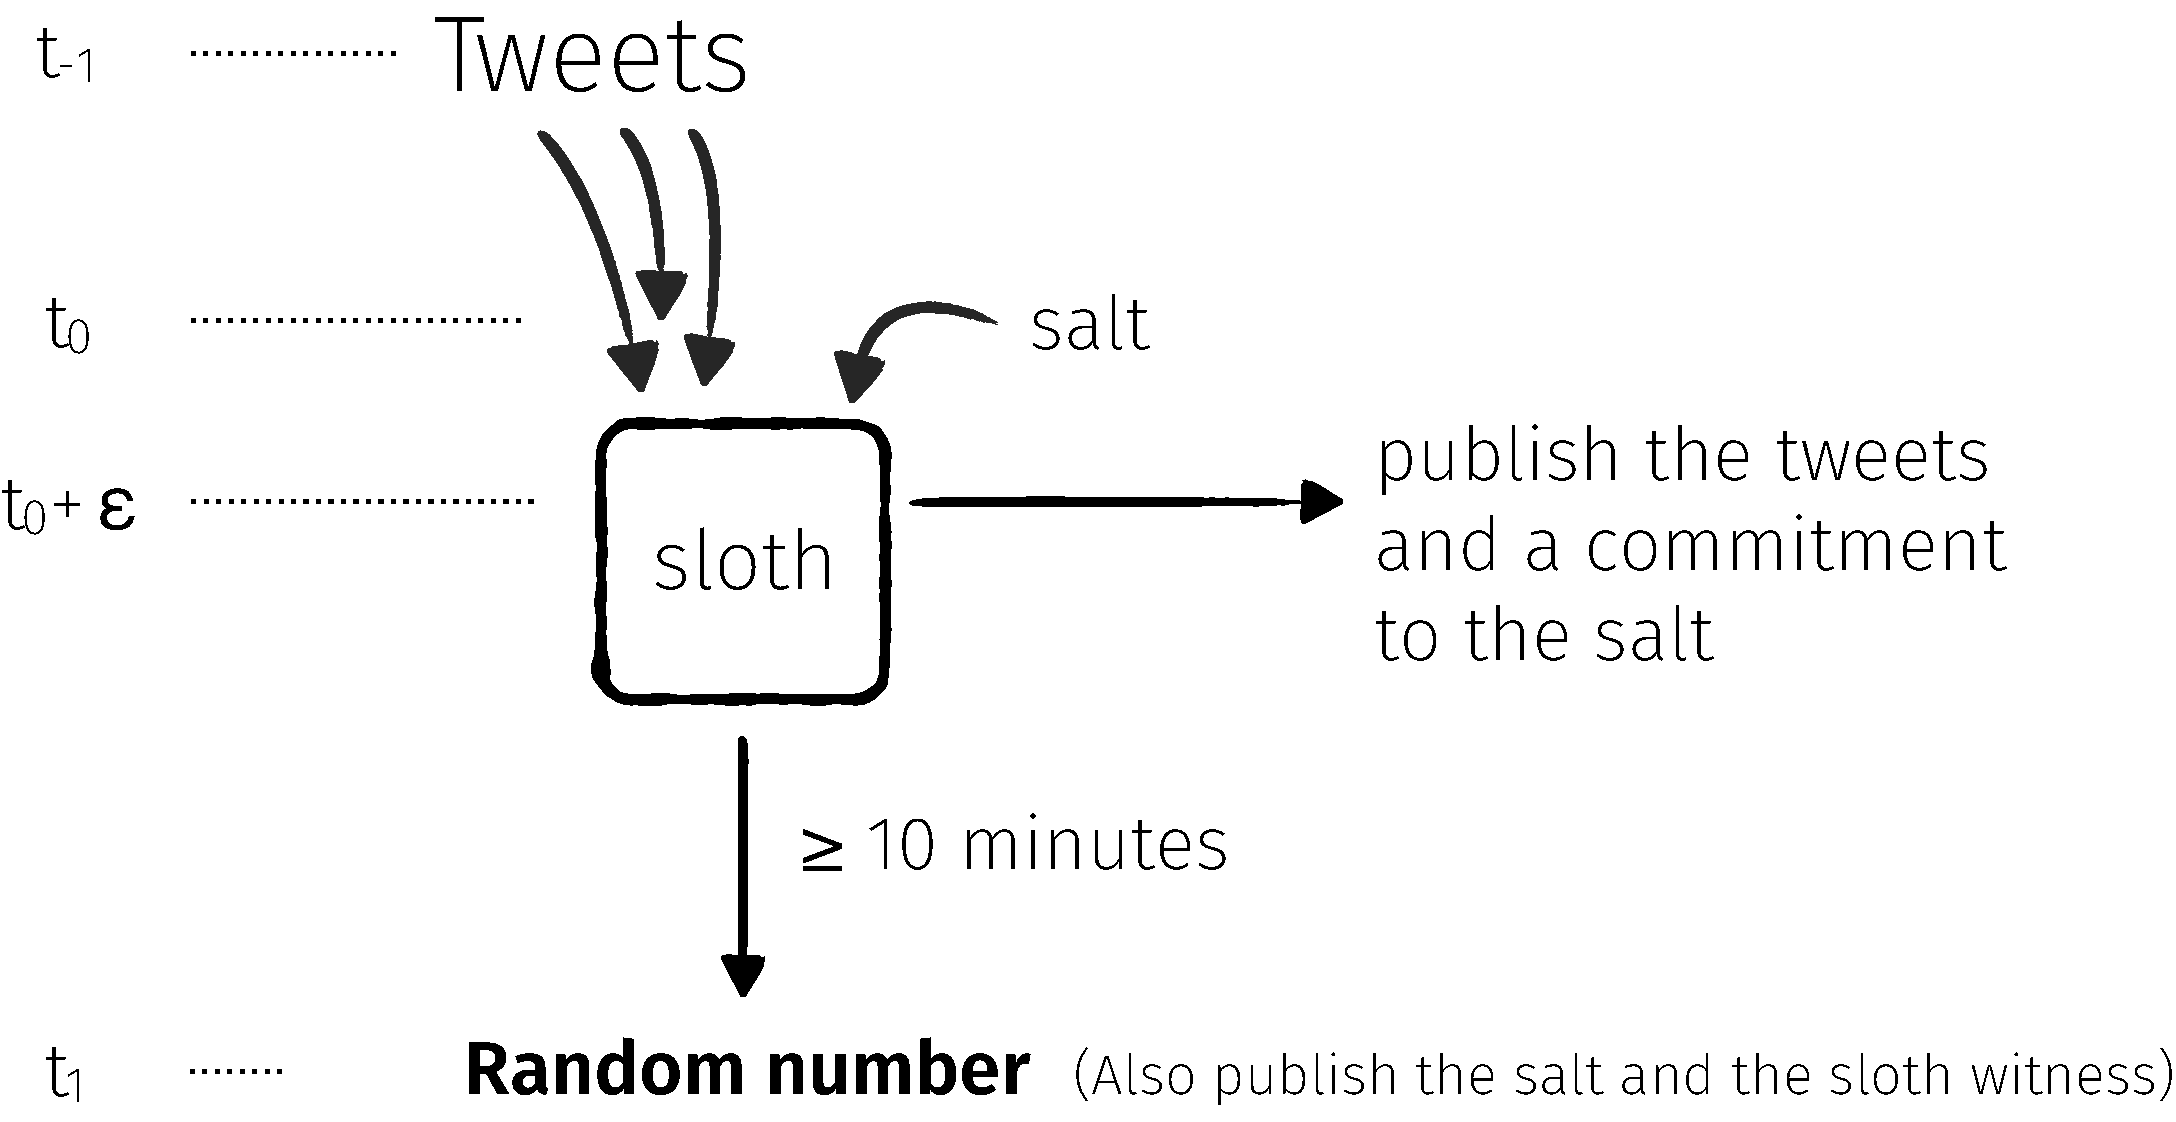
\includegraphics[width=\textwidth]{figures/keep/ARandomZoo.pdf}
        \end{column}
        \begin{column}{0.3\textwidth}
            \begin{center}
                \scalebox{0.85}{
                \begin{tikzpicture}[auto]
                    \pgfdeclarelayer{background}
                    \pgfsetlayers{background,main}
                    \node[block] (input) {Verifiable input};
                    \node[block, below=1cm of input] (computation) {Computation\\$f(I_t)$};
                    \node[block, below=1cm of computation] (users) {Users};
                    \draw[arrow] (input) -- node[yshift=1mm] (inp) {$I_t$} (computation);
                    \draw[arrow] (computation) -- node[yshift=-1mm] {$O_t$} (users);
                    \begin{pgfonlayer}{background}
                        \node[block] (beacon) [container, fill=GoogleBlueGrey!40, draw=GoogleBlueGrey, fit={(computation)}] {};
                    \end{pgfonlayer}
                \end{tikzpicture}
                }
             \end{center}
        \end{column}
        \end{columns}
\end{frame}
\note{
    \begin{itemize}

				\item $t_{-1}$: \textbf{Data reception starts}.
				\begin{itemize}
					\item Concatenated in order of arrival.

				\end{itemize}
				\item $t_0$: \textbf{Data reception stops}
				\begin{itemize}
					\item After a small \textbf{epsilon} (less than a second), the concatenated tweets and a commitment to salt published.
					\item Sloth is started on\textbf{ tweets concatenated with salt}.
					\item Sloth is just a\textbf{ hash function} that is very slow.
				\end{itemize}
				\item $t_1$ The result of the sloth is the hash.
				\begin{itemize}
					\item the salt is published
					\item and the \textbf{witness is a shortcut} to verification.
				\end{itemize}
				\item Any user should try to tweet as close to $t_0$ as possible to make sure $t_0$ is the deadline.
    \end{itemize}

}

\begin{frame}{Trustless Randomness Beacons}
    %\newlength{\onethird}
    \setlength{\onethird}{0.315\textwidth}
    \vspace{.2cm}
    \begin{minipage}[t]{\onethird}
        \centering
        \textbf{Autocratic Collector\vphantom{j}}\\
        %\vspace{.6cm}
        \huge\color[rgb]{1,0,0} $\times$
    \end{minipage}
    ~~\begin{minipage}[t]{\onethird}
        \centering
        \textbf{Specialized MPC}\\
        \begin{itemize}
					\item Scalability Issues
					\item All participants must actively participate
				\end{itemize}
    \end{minipage}
    ~~\begin{minipage}[t]{\onethird}
        \centering
        \textbf{Transparent Authority}\\
				\begin{itemize}
					\item Simpler construction
					\item (Potentially) Single point of failure
				\end{itemize}
    \end{minipage}
\end{frame}
\note{
    \begin{itemize}
				\item Autocratic Collector
				\begin{itemize}
					\item Obviously not ideal for us. Not able to trust it.
				\end{itemize}
				\item Specialized MPC
				\begin{itemize}
					\item The most \textbf{complex}
					\item Security governed by heavy\textbf{ math, cryptography and protocols}
					\item \textbf{Scalability} issues that needs to be solved
					\item Must participate by \textbf{``being there'' and do work}
					\item POSS: Best suited for permissioned settings
				\end{itemize}
        \item Transparent Authority
				\begin{itemize}
					\item (where s-mpc governed by math) Governed by simpler things such as \textbf{logic}, like the slow hash functions in Random Zoo.
					\item So often simpler
					\item Often being a \textbf{single authority}, \textbf{single point of failure}
				\end{itemize}
    \end{itemize}
}

